\documentclass[a4paper,fleqn]{cas-sc}
\usepackage[square,comma,numbers,sort&compress]{natbib}
\usepackage{bm}
\usepackage[]{hyperref}
% \usepackage{calrsfs}
\usepackage[font=small,labelfont=bf]{caption}

\newcommand\ket [1] {|#1 \rangle }
\newcommand\bra [1] {\langle #1 |}
\newcommand{\bracket}[2]   {  \left<#1 |  #2\right>}
\newcommand{\av}[1]{\langle #1\rangle}
\newcommand{\bb}[1]{\mathbf{#1}}

% Short title
\shorttitle{TSAHDU}    

% Short author
\shortauthors{\textit{Waajacu}}  

\begin{document}
\let\WriteBookmarks\relax
\def\floatpagepagefraction{1}
\def\textpagefraction{.001}

\title[mode = title]{TSAHDU: Open Source Expert System for Law, \\Vector Representation of Meaning in Judicial Searches}

%\tnotemark[1,2]

%\tnotetext[1]{This document is the results of the research project
   % funded by the National Science Foundation.}

  %\tnotetext[2]{The second title footnote which is a longer text
    %matter to fill through the whole text width and overflow into
    %another line in the footnotes area of the first page.}

  \author[1]{\textit{Waajacu}}[orcid=0000-0001-6386-9350]
  \cormark[1] 
  %\fnmark[1] 
  \ead{savethebeesandseeds@gmail.com} 
  \ead[url]{www.waajacu.com}

  %\credit{Conceptualization of this study, Methodology, Software}

  \address[1]{Santiago Restrepo Ruiz, Colombia.}

  \cortext[cor1]{Corresponding author} 
  %\cortext[cor2]{Principal corresponding author} 
  %\fntext[fn1]{This is the first author footnote. 
    %but is common to third author as well.}

  %\fntext[fn2]{Another author footnote, this is a very long footnote
    %and it should be a really long footnote. But this footnote is not
    %yet sufficiently long enough to make two lines of footnote text.}

  %\fntext[fn3]{K. Berry is the editor of \TeX Live.}

  %\nonumnote{This note has no numbers. I}

\begin{abstract}
  Non weaponizable research the sort of Law and Market requires caution and broadcasting easy to use interfaces. 
  Market is being still stabilized for a broad and stable theoretical common fortune of all commendable participants. 
  Effective and broad access to Law however is intended in this paper; To be distributed and used without cost: 
  \href{https://github.com/savethebeesandseeds/tsahdu}{https://github.com/savethebeesandseeds/tsahdu}
  
\end{abstract}
 \begin{keywords}
  Law, Open Source, Search Engine, Expert System, Transformers, Natural Language Processing, Neural Networks, NLP, NLU, Colombia. 
 \end{keywords}

 \maketitle
%\linenumbers

\section{Introduction}
Exercise a natural advice of caution those doing advanced Mathematics, an assertive guide not to risk a weaponizable tool. 
Laws sort a encyclopedic strength, prerogative of these with aims to reduce the barrier of 
knowledge and the price of legal advice; a tool on perpetuity free and with open access. 
\noindent
The method serves to consult the state of Law and the state of Jurisprudence, 
given a Text describing a situation; Tsahdu is a modern search engine dedicated to Law. 
Implementation is for now limited to the sovereign Constitution and the sovereign Codes of Law of the Republic of Colombia. 

\section{Mathematical Background}
Used basis are, real numbers: $\mathbb{R}$, integers: $\mathbb{Z}$. To represent a phrases in Human language: $\mathbb{W}$. 
And a reference in a document of Law: $\mathbb{Q}$. Here a scalar $v$ is specified to be real if ${}_{\mathbb{R}}v$ and a 
$p$-dimensional real vector is defined as: ${}_{\mathbb{R}^{p}}V$. Multiple vectors are grouped like Tensors, 
$m$ grouped vectors is defined as ${}_{\mathbb{R}^{p}}V^{m}$.\\
\noindent
Reference to a \textit{document of Law} discriminates $n$ individual Articles ${}_{\mathbb{W}}\mathcal{A}^{n}$. \\

\noindent
Following a static transformation $\phi{}(\cdot)$ each article is represented by a dense vector: 
\begin{equation}
  \begin{split}
    \phi({}_{\mathbb{W}}\mathcal{A}^{n}) \hspace{5pt} &= \hspace{5pt} {}_{\mathbb{R}^{d}}V^{n}.
  \end{split}
\end{equation}
\noindent
Where $\mathbf{V}$ is known as Embedding (in common transformation models $d=384$), 
${}_{\mathbb{W}}\mathcal{A}$ are Article Paragraphs of varying length up to $s=512$ words long, 
$n$ is a positive integer ${}^{+}\mathbb{Z}$ specifying the article index. \\

\noindent
Considering any paragraph or phrase is transformed into a dense vector $\{\mathcal{A}^{n} \rightarrow \mathbf{V}^{n}\}$, 
a document of Law is understood as a dense Matrix ${}_{\mathbb{R}^{n}\times\mathbb{R}^{d}}{\mathbf{M}}$ of size $n\times{d}$. 
Any article larger than $s=512$ words is fragmented and averaged in vector space. \\
\noindent
The aforementioned transformation to vector space $\phi{}(\cdot{})$ is done using \cite{https://doi.org/10.48550/arxiv.1706.03762} implementations: 
\href{https://huggingface.co/}{Natural Language Transformers Models}\footnote{https://huggingface.co/}, on what is known as a 
\href{https://huggingface.co/sentence-transformers/}{Sentence Transformer}\footnote{https://huggingface.co/sentence-transformers/}. 
Whereby two sentences are alike if their vector representation is alike. 


\section{An Expert System for the Law}
Search engines can be modular or anyway very complex, mixing multiple searching methods. 
This expert system description considers only the comparison in vector space. \\
\noindent
A citizen needing advice of Law will query a description paragraph ${}_{\mathbb{W}}\mathcal{U}$, 
the expert system will consider the vector coming from the query transformation $\phi({}_{\mathbb{W}}\mathcal{U})$ 
and compare it against the matrix of Law $\mathbf{M}$. 
Rows most similar with the user query are returned as a reference of Law, note that every row in $\mathbf{M}$ 
has associated a specific reference of Law $\mathbb{Q}$, 
e.g. article number $n$ in chapter $q$, title $u$, book $w$ and document $z$, this is $\mathbb{Q}:<z,w,u,q,n>$.\\

\noindent
Regex expressions are used to separate Articles, discriminate references. 
There is generally one Constitution and many Laws compiled in documents known as Codes. 
Robots automates the downloading and updating of those .pdf documents. 
Further automation extracts the text content of the document and generates regular .txt files; 
Finally using regular Expressions (regex) the full text is separated into individual articles with their associated reference. 

\section{An Expert System for Jurisprudence}
These are Court sentences and resolutions, serves an enormous advantage to the exercise of a Judge and required to provide a 
proper trial. Also to evaluate the cogency for the exercise of Law in a sovereign state. \\

Defining a reference to a sentence of a Court dictum on \textit{Jurisprudence} searches requires the same vector approach $\phi(\cdot)$ 
but a different indexing of phrases, as the division by articles is only found in documents of Law. To generalize 
the technique across different type of documents, the role of $n$ is changed to the role of $\rho$. Where $\rho$ is a positive integer 
${}^{+}\mathbb{Z}$ know as the document density count, it varies from document to document as different documents has different sizes ---
for example, $\rho=100$ implies a document was fragmented into 100 phrases. Creating, 
for every document a matrix ${}_{\mathbb{R}^{\rho}\times\mathbb{R}^{d}}{\mathbf{M}}$.\\

\section{Considerations of Implementation}
Law recommendation is a sensible topic, an online open service requires an explicit caution note specifying a check statement: 
"\color{red}\underline{this is not a professional advice of law}\color{black}". \\
\noindent
The colossal body of Jurisprudence 
and the monumental size of Law, require computational efficiency of implementation, so a high performance programming language is 
recommended. Robotic Web Process Automation is probably required to scrap and update Web documents. 
Transformers Networks are downloaded pretrained for the idiom or matching tongue, further fine tuning is recommended. \\
The sensibility of the topic involve require the Transformer Network be trained properly, 
on a mistake in a case of Law the developers intend to show good faith by maximizing likelihood on the training procedure. \\
.pdf documents are better stored as .txt files, not every .pdf document has a straightforward way to 
transform into a .txt, sometimes software known as optical character recognition is required. \\
Regex as a way to segment files into articles is not very stable, on this part there is still a lot of Human work required. 

\section{Vector Representation of a Phrase}
Law is very well written, but natural language is not precise; The challenge for English is the same challenge for Spanish, 
they have not a straightforward analytical representation $f(\cdot): \mathbb{W}\rightarrow\mathbb{R}^{x}$. 
Best I know how is Deep Learning Transformers $\phi(\cdot): \mathbb{W}\rightarrow\mathbb{R}^{d}$, 
as a way to formulate Text ($\mathbb{W}$) as a precise numeric abstraction ($\mathbb{R}$). \\
A high goal for the sciences of language is to construct and agree on an analytical transformation of idioms to vectors, 
an orthogonal language would serve Humanity with great progress, but it is proven to be very hard, justice is mixed 
with poetry and without extensive context science seems like fantasy. \\

\noindent
Until a transformation is discovered and accord on, best we can do is to use Deep Neural Networks, 
generally known as Text Input Transformers Neural Architecture; Where a specific Layer inside the Deep model 
is used to represent the Input Phrase as a Vector of embedding. \\
\textit{For English Language: \href{https://huggingface.co/sentence-transformers/all-MiniLM-L12-v2}{all-MiniLM-L12-v2}\footnote{https://huggingface.co/sentence-transformers/all-MiniLM-L12-v2} with a vector size $d=384$.}\\
\textit{For Spanish Language: \href{https://huggingface.co/hiiamsid/sentence_similarity_spanish_es}{sentence\_similarity\_spanish\_es}\footnote{https://huggingface.co/hiiamsid/sentence\_similarity\_spanish\_es} with a vector size $d=768$.}\\

There are Transformers for other languages; English Model performs better than Spanish. 
With a sufficient corpus of Law one can fine train any of these Models to better perform. 

\section{Stable Embedding}
These are some marginal operations to better represent the embedding vector: ${}_{\mathbb{R}^{d}}\mathbf{V}$. 
\noindent
It be useful for the vector to be normalized, two types of normalization are consider:
\begin{equation}
  \begin{split}
    \mu_{1}-normalization&:= {}_{\mathbb{R}^{d}}\mathbf{V} = \hspace{8pt} \frac{1}{{}_{\mathbb{R}}\mu_{1}}\cdot{}{}_{\mathbb{R}^{d}}\mathbf{V},\hspace{25pt}
    where: \hspace{8pt} {}_{\mathbb{R}}\mu_{1} = \sum_{i=1}^{d}{}_{\mathbb{R}}\mathbf{V}_{i}
  \end{split}
\end{equation}
\begin{equation}
  \begin{split}
    \mu_{2}-normalization&:= {}_{\mathbb{R}^{d}}\mathbf{V} = \hspace{8pt} \frac{1}{{}_{\mathbb{R}}\mu_{2}}\cdot{}{}_{\mathbb{R}^{d}}\mathbf{V},\hspace{25pt}
    where: \hspace{8pt} {}_{\mathbb{R}}\mu_{2} = \sum_{i=1}^{d}abs({}_{\mathbb{R}}\mathbf{V}_{i})
  \end{split}
\end{equation}
\begin{equation}
  \begin{split}
    \mu_{3}-normalization&:= {}_{\mathbb{R}^{d}}\mathbf{V} = \hspace{8pt} \frac{1}{{}_{\mathbb{R}}\mu_{3}}\cdot{}{}_{\mathbb{R}^{d}}\mathbf{V},\hspace{25pt}
    where: \hspace{8pt} {}_{\mathbb{R}}\mu_{3} = \sqrt{\sum_{i=1}^{d}({}_{\mathbb{R}}\mathbf{V}_{i})^{2}}
  \end{split}
\end{equation}
\noindent
Where $(\cdot{})$ is the element-wise multiplication.\\
\noindent
From now on, unless otherwise mention assume $\mathbf{V}$ and all the rows in $\mathbf{M}$ are $\mu_{3}-normalized$, this is the 
standard way to normalize a vector.\\


\section{Average vector}
A policy for dealing with long phrases is superposition of rolling overlapping windows of 
phrase segments averaged in vector space. The superposition of multiple ($m$) vectors outputs a vector: 
\begin{equation}
  \begin{split}
    {}_{\mathbb{R}^{d}}{Avg}\left(\mathbf{V}^{m}\right) =& \hspace{8pt} \frac{1}{m}\cdot{}\sum_{i=1}^{m} {}_{\mathbb{R}^{d}}\mathbf{V}^{(i)}
  \end{split}
\end{equation}
Where $(\cdot{})$ is the element-wise multiplication, and $\Sigma$ sums vectors. \\
\noindent
In Law, Articles are grouped in Chapters, Chapters are grouped in Titles and all Titles make a Document. 
It is useful to know the average vector of an entire Chapter $({}_{\mathbb{W}}\mathcal{C})$, 
Title $({}_{\mathbb{W}}\mathcal{T})$, Book $({}_{\mathbb{W}}\mathcal{B})$ or Document $({}_{\mathbb{W}}\mathcal{D})$, 
and for long Articles also $({}_{\mathbb{W}}\mathcal{A})$. 
---the vector of it's member phrases average, and so on, 
\begin{equation}
  \begin{split}
    {}_{\mathbb{R}^d}\phi({}_{\mathbb{W}}\mathcal{A}^{n}) =& \hspace{8pt} {Avg}\left(\mathbf{V}^{m}\right), \hspace{10pt} \forall m \in \mathcal{A}^{n}, \hspace{25pt} \textsf{average vector over all phrases in the nth-article}\\
    {}_{\mathbb{R}^d}\phi({}_{\mathbb{W}}\mathcal{C}^{q}) =& \hspace{8pt} {Avg}\left(\mathbf{V}^{m}\right), \hspace{10pt} \forall m \in \mathcal{C}^{q}, \hspace{28pt} \textsf{average vector over all phrases in the qth-chapter}\\
    {}_{\mathbb{R}^d}\phi({}_{\mathbb{W}}\mathcal{T}^{u}) =& \hspace{8pt} {Avg}\left(\mathbf{V}^{m}\right), \hspace{10pt} \forall m \in \mathcal{T}^{u}, \hspace{25pt} \textsf{average vector over all phrases in the uth-title}\\
    {}_{\mathbb{R}^d}\phi({}_{\mathbb{W}}\mathcal{B}^{w}) =& \hspace{8pt} {Avg}\left(\mathbf{V}^{m}\right), \hspace{10pt} \forall m \in \mathcal{B}^{w}, \hspace{25pt} \textsf{average vector over all phrases in the wth-book}\\
    {}_{\mathbb{R}^d}\phi({}_{\mathbb{W}}\mathcal{D}) =& \hspace{8pt} {Avg}\left(\mathbf{V}^{m}\right), \hspace{10pt} \forall m. \hspace{25pt} \textsf{average vector over all phrases in the document}
  \end{split}
\end{equation}

Those are meant to be simple formulas, but imply some considerations; let me explain by a simple example: 
Imagine a window size of $s=2$ words and overlapping of size $g=1$, the user inputs this phrase: \\
${}_{\mathbb{W}}$"\color{brown}Dogs chase Cats\color{black}" 
$\rightarrow$ 
\textbf{[}${}_{\mathbb{W}}$"\color{brown}Dogs chase\color{black}",${}_{\mathbb{W}}$"\color{brown}chase Cats\color{black}"\textbf{]} 
$=\textbf{[}{}_{\mathbb{R}^d}\textbf{[}\color{brown}2.0,3.0,1.0,...\color{black}\textbf{]}, 
{}_{\mathbb{R}^d}\textbf{[}\color{brown}4.0,5.0,6.0,...\color{black}\textbf{]}\textbf{]}$, \\
${}_{\mathbb{W}}$"\color{brown}Dogs chase Cats\color{black}" = ${}_{\mathbb{R}^d}\textbf{[}\color{brown}3.0,4.0,3.5,...\color{black}\textbf{]}$\\

\noindent
Since the phrase was too long, the overlapping window policy segmented the input phrase into two partial phrases. 
The result is the average vector, consider to think the embedding for the word in the middle 
${}_{\mathbb{W}}$"\color{brown}\textit{chase}\color{black}" was considered two times, this is not ideal. \\

If $s=2$ and there is no overlap considered $g=0$, contextual information might be broken: \\
${}_{\mathbb{W}}$"\color{brown}Dogs chase Cats\color{black}" 
$\rightarrow$ 
\textbf{[}${}_{\mathbb{W}}$"\color{brown}Dogs chase\color{black}",${}_{\mathbb{W}}$"\color{brown}Cats\color{black}"\textbf{]} 
$=\textbf{[}{}_{\mathbb{R}^d}\textbf{[}\color{brown}2.0,3.0,1.0,...\color{black}\textbf{]}, 
{}_{\mathbb{R}^d}\textbf{[}\color{brown}1.0,0.5,9.0,...\color{black}\textbf{]}\textbf{]}$, \\
${}_{\mathbb{W}}$"\color{brown}Dogs chase Cats\color{black}" = ${}_{\mathbb{R}^d}\textbf{[}\color{brown}1.5,1.75,5.0,...\color{black}\textbf{]}$\\

\noindent
The two approaches yield different average vectors, this trade-off is hard to come-by. \\
Values of $s=512$ and $g=64$, seem to work fine. \\ 

\section{Dense Vectors Comparison}
Be sure any vector $\mathbf{V}$ is normalized in it self: 
$\mathbf{V}=||{\mathbf{V}^{*}}||^{-1}\cdot{}\mathbf{V}^{*}$ so that, $\sum_{j=1}^{d}V_{j}=1$.\\
Comparing two vectors, vector $({}_{\mathbb{R}^{d}}\mathbf{V}_{a}=a)$ and $({}_{\mathbb{R}^{d}}\mathbf{V}_{b}=b)$, 
these are some simple comparison formulas: 
\begin{equation}
\begin{split}
  Minkowski: & \hspace{25pt} \left(\sum_{j=1}^{d}(a_{j}-b_{j})^p\right)^{1/p} \\
  Cosine: & \hspace{25pt} \frac{\sum_{j=1}^{d}a_{j}\cdot{}b_{j}}{\sqrt{\sum_{j=1}^{d}(a_{j})^2}\cdot{}\sqrt{\sum_{j=1}^{d}(b_{j})^2}} \\
  Dot-Product: &\hspace{25pt} \sum_{j=1}^{d}a_{j}\cdot{}b_{j}
\end{split}
\end{equation}
Where ${}_{\mathbb{R}}a_{j}$ and ${}_{\mathbb{R}}b_{j}$ are the scalar components in the j index of the vectors 
$_{\mathbb{R}^{d}}\mathbf{V}_{a}$ and $_{\mathbb{R}^{d}}\mathbf{V}_{b}$ respectably. For Dot-Product and Cosine, 
the higher the value the better, for Minkowski the lower the value the better. \\
Euclidean distance, arise from Minkowski where $p=2$. However, the size for the dense vector is very high $d=384$, 
the overall information from the upmost relevant dimensions might be opaqued given the vector size, 
to illustrate this let's view in the Figure \ref{fig1} below: \\

\begin{figure}[!h]
  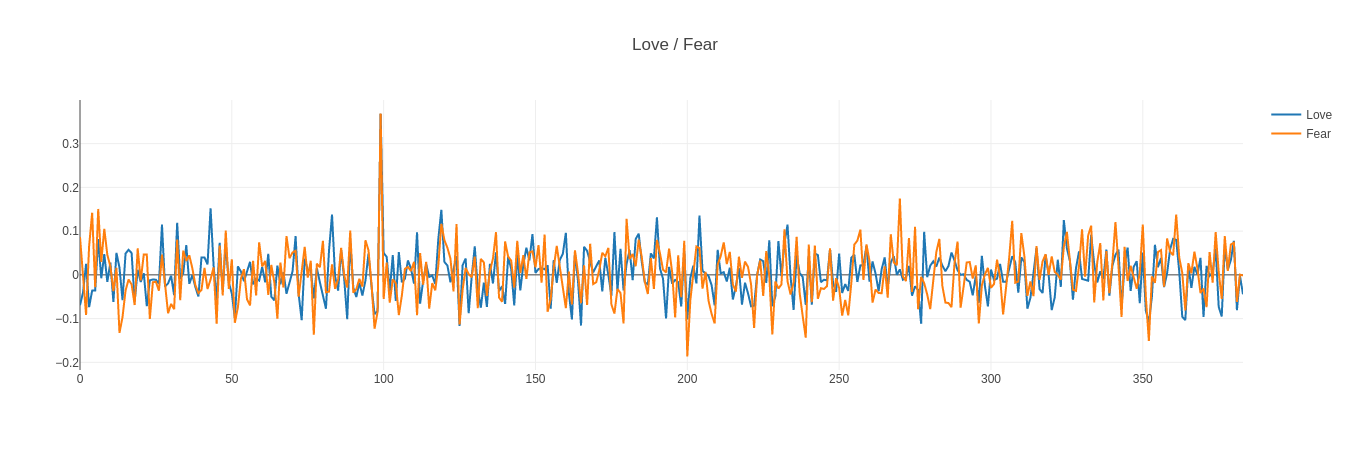
\includegraphics[width=\textwidth,height=\textheight,keepaspectratio]{./images/love_fear}
  \captionof{figure}{Embedding Vectors for the words \textbf{\textit{Love}} and \textbf{\textit{Fear}}, 
  To be notice index 99 might be a flag for the Human emotion component. The numeric comparison yields are: 
  Minkowski(p=1): 0.13416162, Minkowski(p=2): 1.0309231, Minkowski(p=3): 0.21693337, Minkowski(p=5): 0.19361636, 
  Cosine: 0.4685991 [rad]. Dot-Product: 0.4685991. These two ideas are as expected fairly different, as the vectors are $\mu_{3}-normalized$ 
  the maximum possible distance using Minkowski(p=2) is 2.0.}
  \label{fig1}
\end{figure}

\noindent
About dense high dimensional vector comparison one might go beyond simple analytical formulas; to train a machine learning comparison 
schema, derive Principal Component Analysis or Relevance Vector Machines to reduce the $d$-dimensional of the vectors. 
Or describe optimization procedures, label or in anyway train a Model to compare vectors. For now the Euclidean distance suffice, 
on these sensible topics efforts rather help to construct analytical solutions, as it is hard to argue the validity of a 
solution involving deep compositional function approximations, like Neural Networks. \\

\noindent
To end the section, let me be simple about it; if every Article is transform into a Vector and a corpus of Law is a Matrix. 
A user input is transformed and compared against the matrix of Law $\mathbf{M}$, returning the references 
of Law corresponding to the rows indices with the lower distance. 

\newpage
\section{Entropy, Information of the Vector Space}
In this framework, Entropy of a Text Fragment is the Entropy of a Layer in a Natural Language Transformer Neural Network. 
This is to say, Entropy of a Text is for this framework the Entropy of the Embedding Vector. 

\noindent
Entropy might be in units of $[Shannon]$ (or $[bits]$) if $log_{2}$ is used, or in units of $[nats]$ if $log_{e}$. 
Let's use the $[Shannon]$ terminology to share respect. Vector Space Entropy usefulness insights about the information 
of a given fragment of Text depends on the method used to train the Transformer Network. 
Experiments for the used Transformer yield \color{brown}not determinant results\color{black}. 

\noindent
A way to calculate Entropy of a Phrase in Vector Space is shown, requires three steps: \\

\noindent
Assert that the Vector is $\mu_{3}-normalized$. \\

\noindent
Have the Vector resemble a Discrete Distribution, on this case let's simply calculate the absolute value in all the dimensions of the vector: 
\begin{equation}\label{eq_ent_1}
  \begin{split}
    {}_{\mathbb{R}^{d}}\mathbf{V}^{*}_{j}&=\hspace{5pt}abs({}_{\mathbb{R}^{d}}\mathbf{V}_{j})\\
  \end{split}
\end{equation}
Finally the Entropy is: \\
\begin{equation}
  \begin{split}
    _{\mathbb{R}}\mathbf{H}_{\mathbf{V}}&=\hspace{5pt} (-1) \cdot{}\sum_{j=1}^{d}\mathbf{V}^{*}_{j}*log_{2}(\mathbf{V}^{*}_{j})\hspace{8pt} [Shannon]  
  \end{split}
\end{equation}
Again, this yield \color{brown}not determinant results\color{black}. The problem is that the Dense vector is defined over positive and negative real numbers, 
a better way to perform the operation in equation \ref{eq_ent_1} will unlock the whole science of information theory. On research I try on with building 
parametric distributions, and also try on having the negative values be a separated distribution and compute the join Entropy, but had no significant results. 
Maybe the solution be on changing the Network Architecture and training with Cross Entropy. 

\newpage
\section{Results}
Implemented in Rustc Language for the Colombian Constitution and for the Colombian Codes of Law in the Republic. 
Source code is available with open access at \href{https://github.com/savethebeesandseeds/tsahdu}{https://github.com/savethebeesandseeds/tsahdu}. 
A demo server was mounted and hosted locally \href{http://www.waajacu.com}{http://www.waajacu.com}. \\

Achieve a high velocity and a stable implementation 
using a Spanish Language Transformer \href{https://huggingface.co/hiiamsid/sentence_similarity_spanish_es}{sentence\_similarity\_spanish\_es} 
with a maximum phrase size of $s=512$ words and overlapping of $g=64$ words.

Complications on gathering the data, .txt files for all Codes of Law and .txt file Article segmentation. 

\section{Future Work}
Refine the current work, implement for other languages and for other countries. 
A better comprehension for the Entropy of the Vector Space will suffice the base for all the information analytics. 

\section{Acknowledgments}
This work was not granted any private or public founds. Research and development was intended for non profit and was done by Waajacu. 
All the mistakes are my own, to be acknowledge are the Mathematicians who developed the state of the Art for Natural Language Understanding 
and the cooperation of Machines. 

\bibliographystyle{is-unsrt}
\bibliography{mybibfile}

\end{document}